% NOTE: must be run with
% xelatex -shell-escape 6_834j_talk
\documentclass[10pt, compress]{beamer}

\usetheme{m}

\usepackage{booktabs}
\usepackage[scale=2]{ccicons}
\usepackage{minted}

\usepgfplotslibrary{dateplot}

\usemintedstyle{trac}

\usepackage{pifont}% http://ctan.org/pkg/pifont
\newcommand{\cmark}{\ding{51}}%
\newcommand{\xmark}{\ding{55}}%

\newcommand{\defeq}{\mathrel{\overset{\makebox[0pt]{\mbox{\normalfont\tiny\sffamily def}}}{=}}}

\title{Robot grocery shopping in partially observable settings}
\subtitle{}
\date{May 13, 2015}
\author{Rodrigo Gomes, Xiaomin Wang, Dustin Tran}
\institute{MIT, 6.834j Cognitive Robotics}

\begin{document}

\maketitle

\begin{frame}[fragile]
  \frametitle{Outline}

  \begin{enumerate}
  \item (2 min) Background on POMDPs, belief-state MDP, MDP solvers we have
  \item (2 min) Setup: Grocery shopping as planning in a POMDP
  \item (4 min) Demo
  \item (2 min) The solver actually used (value iteration)
  \item (1 min) Things that failed (Thompson sampling)
  \item (1 min) Q\&A
  \end{enumerate}
\end{frame}

\begin{frame}[fragile]
  \frametitle{Partially observable Markov decision process (POMDPs)}

  Collection of objects $(S,A,\Omega,R,T,O)$

  \begin{itemize}
  \item $S$: state space
  \item $A$: action space
  \item $\Omega$: observation space
  \item $T$: transition operator. $T(s' \mid s,a)$ is probability of next state $s'$ given state $s$ and action $a$
  \item $O$: observable operator. $O(o \mid s)$ is probability of observing
  $o$ given at state $s$
  \item $R: S \times A \rightarrow \mathbb{R}$ reward function
  \end{itemize}
\end{frame}

\begin{frame}[fragile]
  \frametitle{Partially observable Markov decision process (POMDPs)}

  \begin{figure}[ht]
  \begin{center}
  \centerline{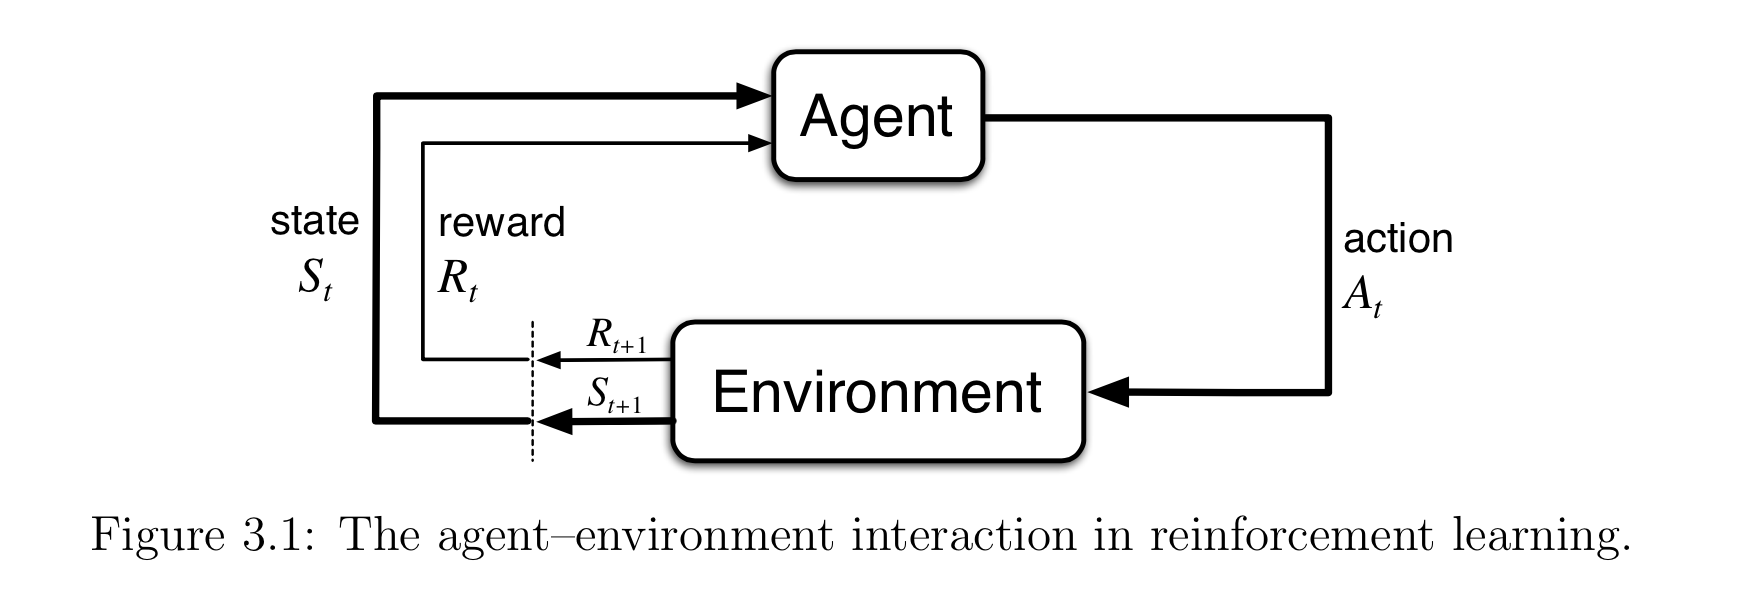
\includegraphics[width=1.5\textwidth]{img/agent_environment.png}}
  \end{center}
  \end{figure}
\end{frame}

\begin{frame}[fragile]
  \frametitle{Grocery shopping}

  the task in the POMDP framework
\end{frame}

\plain{demo}

\begin{frame}[fragile]
  \frametitle{Demo}

  link from here to a bunch of videos and an interactive demo
\end{frame}

\begin{frame}[fragile]
  \frametitle{Results}

  the task in the POMDP framework
\end{frame}

\plain{
  {\Large Play with it!}\\[5ex]
  
\includegraphics{img/octocat.png}\\[3ex]
  github.com/dustinvtran/bayesrl
}

\end{document}
